\documentclass[11pt,professionalfonts,hyperref={pdftex,pdfpagemode=none,pdfstartview=FitH}]{beamer}
%\usepackage{times}
%\usefonttheme{serif}
%\usepackage{helvet}
%\usepackage{amsmath,amssymb}
\usepackage{graphicx,multirow}
\usepackage[scriptsize]{subfigure}
\usepackage{epstopdf}
\usepackage{multimedia}
\usepackage{hyperref}

%\usepackage{media9}


% movie sty

%\usepackage{movie15}

%\usepackage{warmread}
%\usepackage[all,import]{xy}

%\renewcommand\mathfamilydefault{\rmdefault}

\newcommand{\norm}[1]{\ensuremath{\left\| #1 \right\|}}
\newcommand{\bracket}[1]{\ensuremath{\left[ #1 \right]}}
\newcommand{\braces}[1]{\ensuremath{\left\{ #1 \right\}}}
\newcommand{\parenth}[1]{\ensuremath{\left( #1 \right)}}
\newcommand{\pair}[1]{\ensuremath{\langle #1 \rangle}}
\newcommand{\met}[1]{\ensuremath{\langle\langle #1 \rangle\rangle}}
\newcommand{\refeqn}[1]{(\ref{eqn:#1})}
\newcommand{\reffig}[1]{Fig. \ref{fig:#1}}
\newcommand{\tr}[1]{\mathrm{tr}\ensuremath{\negthickspace\bracket{#1}}}
\newcommand{\trs}[1]{\mathrm{tr}\ensuremath{[#1]}}
\newcommand{\deriv}[2]{\ensuremath{\frac{\partial #1}{\partial #2}}}
\newcommand{\SO}{\ensuremath{\mathsf{SO(3)}}}
\newcommand{\T}{\ensuremath{\mathsf{T}}}
\renewcommand{\L}{\ensuremath{\mathsf{L}}}
\newcommand{\so}{\ensuremath{\mathfrak{so}(3)}}
\newcommand{\SE}{\ensuremath{\mathsf{SE(3)}}}
\newcommand{\se}{\ensuremath{\mathfrak{se}(3)}}
\renewcommand{\Re}{\ensuremath{\mathbb{R}}}
\newcommand{\aSE}[2]{\ensuremath{\begin{bmatrix}#1&#2\\0&1\end{bmatrix}}}
\newcommand{\ase}[2]{\ensuremath{\begin{bmatrix}#1&#2\\0&0\end{bmatrix}}}
\newcommand{\D}{\ensuremath{\mathbf{D}}}
\newcommand{\Sph}{\ensuremath{\mathsf{S}}}
\renewcommand{\S}{\Sph}
\newcommand{\J}{\ensuremath{\mathbf{J}}}
\newcommand{\Ad}{\ensuremath{\mathrm{Ad}}}
\newcommand{\intp}{\ensuremath{\mathbf{i}}}
\newcommand{\extd}{\ensuremath{\mathbf{d}}}
\newcommand{\hor}{\ensuremath{\mathrm{hor}}}
\newcommand{\ver}{\ensuremath{\mathrm{ver}}}
\newcommand{\dyn}{\ensuremath{\mathrm{dyn}}}
\newcommand{\geo}{\ensuremath{\mathrm{geo}}}
\newcommand{\Q}{\ensuremath{\mathsf{Q}}}
\newcommand{\G}{\ensuremath{\mathsf{G}}}
\newcommand{\g}{\ensuremath{\mathfrak{g}}}
\newcommand{\Hess}{\ensuremath{\mathrm{Hess}}}
\newcommand{\refprop}[1]{Proposition \ref{prop:#1}}

\definecolor{mygray}{gray}{0.9}

\mode<presentation> {
  \usetheme{Warsaw}
  \usefonttheme{serif}
  \setbeamercovered{transparent}
}

\newcommand{\mypaper}{}

\setbeamertemplate{footline}%{split theme}
{%
  \leavevmode%
  \hbox{\begin{beamercolorbox}[wd=.76\paperwidth,ht=2.5ex,dp=1.125ex,leftskip=.3cm,rightskip=.3cm plus1fill]{author in head/foot}%
    \usebeamerfont{author in head/foot}\insertshorttitle
  \end{beamercolorbox}%
  \begin{beamercolorbox}[wd=.24\paperwidth,ht=2.5ex,dp=1.125ex,leftskip=.3cm,rightskip=.3cm]{title in head/foot}
%    \usebeamerfont{title in head/foot}\mypaper\hfill \insertframenumber/\inserttotalframenumber
    \usebeamerfont{title in head/foot}\hfill \insertframenumber/\inserttotalframenumber
  \end{beamercolorbox}}%
  \vskip0pt%
} \setbeamercolor{box}{fg=black,bg=yellow}

\title[Design and Development of a Free-Floating Hexrotor UAV for 6-DOF Maneuvers]{\large Design and Development of a Free-Floating\\Hexrotor UAV for 6-DOF Maneuvers}

\author{\vspace*{-0.3cm}}

\institute{\footnotesize
{\normalsize Evan Kaufman, Kiren Caldwell,\\Daewon Lee, and Taeyoung Lee}\vspace*{0.2cm}\\
  Mechanical and Aerospace Engineering\\ The George Washington University}

\date{}

\definecolor{tmp}{rgb}{0.804,0.941,1.0}
\setbeamercolor{numerical}{fg=black,bg=tmp}
\setbeamercolor{exact}{fg=black,bg=red}

\newtheorem{prop}{Proposition}



\renewcommand{\emph}[1]{\textit{\textbf{\color{blue}{#1}}}}


\begin{document}

\begin{frame}
  \titlepage
\end{frame}


\section*{}
\subsection*{Introduction}

\begin{frame}
\frametitle{Introduction}
\framesubtitle{Spacecraft Maneuvers and Limitations}
\begin{itemize}
    \item Spacecraft rotational maneuvers
    \begin{itemize}
    	\item Examples: relative orientation in formation, detumbling
    	\item Attitude maneuvers may involve large rotational trajectories over long time periods
	\item Motivation: develop an experimental testbed for rotational maneuvers before controllers are applied to spacecraft
    \end{itemize}
    \item Restrictions of attitude controlled testbeds
	\begin{itemize}
	\item Spherical air bearings exhibit severe rotational restrictions
	\item Quadrotor UAVs are constrained to a single attitude plane for hovering and are underactuated
	\end{itemize}
\end{itemize}

\only<1->{
\begin{figure}
\centerline{
    \includegraphics[height=2.5cm]{SFCN.pdf}\hspace*{0.5cm}
    \includegraphics[height=2.5cm]{SphericalAirBearing}\hspace*{0.5cm}
    \includegraphics[height=2.5cm]{quadrotor}
}
\end{figure}}

\end{frame}


\begin{frame}
\frametitle{Motivation}
\framesubtitle{Rotational Manuever Testbed}

\begin{itemize}
	\item Free-floating UAV
	\begin{itemize}
	\item No support restrictions like that of spherical air bearing
	\item Capable of large angle rotations over prolonged time periods
	\end{itemize}
\vspace*{0.3cm}\pause
	\item Fully-actuated UAV
	\begin{itemize}
	\item Control of six translational and rotational degrees of freedom
	\item Requirement to produce a force and a moment in any direction
	\item Hover may be possible over a wide range of attitudes
	\end{itemize}
\end{itemize}

\end{frame}


\section*{}
\subsection*{Hardware and Software}

\begin{frame}
\frametitle{Hexrotor UAV Development}
\framesubtitle{Reference Frames and Propeller Layout}

\begin{itemize}
	\item Multi-planar Propeller Layout
	\begin{itemize}
	\item Two propellers opposite each other share the same plane
	\item Each set of opposite counter-rotating propellers produces a thrust in one dimension and a moment in one dimension
	\item Neighboring propellers occupy orthogonal planes; UAV arms lie on the same plane
	\item The vector sum of forces and moments of three propeller pairs allow for force and moment in \emph{any} direction
	\end{itemize}
\item (Number of actuators)$=$(Number of degrees of freedom); position and attitude tracking are completely decoupled

\only<1->{
\begin{figure}
\centerline{
    \includegraphics[height=2.5cm]{b_to_t}\hspace*{1cm}
    \includegraphics[height=2.5cm]{e_to_b}
    \vspace*{0.5cm}
}
\end{figure}}
\end{itemize}
\end{frame}




\begin{frame}
\frametitle{Hexrotor UAV Development}
\framesubtitle{Actuation}

\begin{itemize}
\item Variable Pitch Propellers
	\begin{itemize}
	\item Capable of producing thrust in two directions
	\item Very fast response time
	\end{itemize}
\vspace*{0.3cm}\pause
\item High Efficiency Actuation
	\begin{itemize}
	\item An accurate estimation of the propeller dynamics are required for control
	\item Motor speed and pitch angle may be controlled individually
	\item A test stand measures the force or torque of the propellers, depending on orientation
	\item Propeller speeds and pitch angles are tested to choose a linear coupling passing through a high-efficiency region
	\end{itemize}

\only<1->{
\begin{figure}
\centerline{
    \includegraphics[height=2cm]{TestStand_Thrust}\hspace*{0.5cm}
    \includegraphics[height=2cm]{TestStand_Moment}\hspace*{0.5cm}
    \includegraphics[height=2cm]{ContoursThrustServo}
\vspace*{0.5cm}
}
\end{figure}}

\end{itemize}
\end{frame}




\begin{frame}
\frametitle{Hardware Structure}

\centerline{
\begin{minipage}[t]{0.5\columnwidth}
\begin{itemize}
    \item Gumstix Computer\\-on-Module (COM)
    \item Propeller I$^2$C commands are executed to brushless DC (BLDC) motors and servo motors (pitch)
    \item Vicon cameras provide position and attitude, sent via XBee communication
    \item Onboard inertial measurement unit (IMU) provides angular velocity
    \item Commercial frame with tubular arms
\end{itemize}
\end{minipage}
%\hspace*{0.1\columnwidth}
\begin{minipage}[t]{0.5\columnwidth}
\only<1->{
\begin{figure}
\centerline{
    \includegraphics[width=5cm]{HardwareSchematic.pdf}
\vspace*{0.5cm}
}
\centerline{
    \includegraphics[height=2.5cm]{ESCsIMU}
\vspace*{0.5cm}
}
\end{figure}}
\end{minipage}
}
\end{frame}

\begin{frame}
\frametitle{Software Structure}

\centerline{
\begin{minipage}[t]{0.5\columnwidth}
\begin{itemize}
    \item Multi-thread structure allows for communication of multiple devices at different rates
    \item Three threads
    \begin{enumerate}
	\item Keyboard command execution via WiFi for various trajectories
	\item Vicon measurements of position and attitude from XBee
	\item IMU data is read and control computed and executed
    \end{enumerate}
\end{itemize}
\end{minipage}
%\hspace*{0.1\columnwidth}
\begin{minipage}[t]{0.5\columnwidth}
\only<1->{
\begin{figure}
\centerline{
    \includegraphics[width=5cm]{SoftwareSchematic.pdf}
\vspace*{0.5cm}
}
\centerline{
    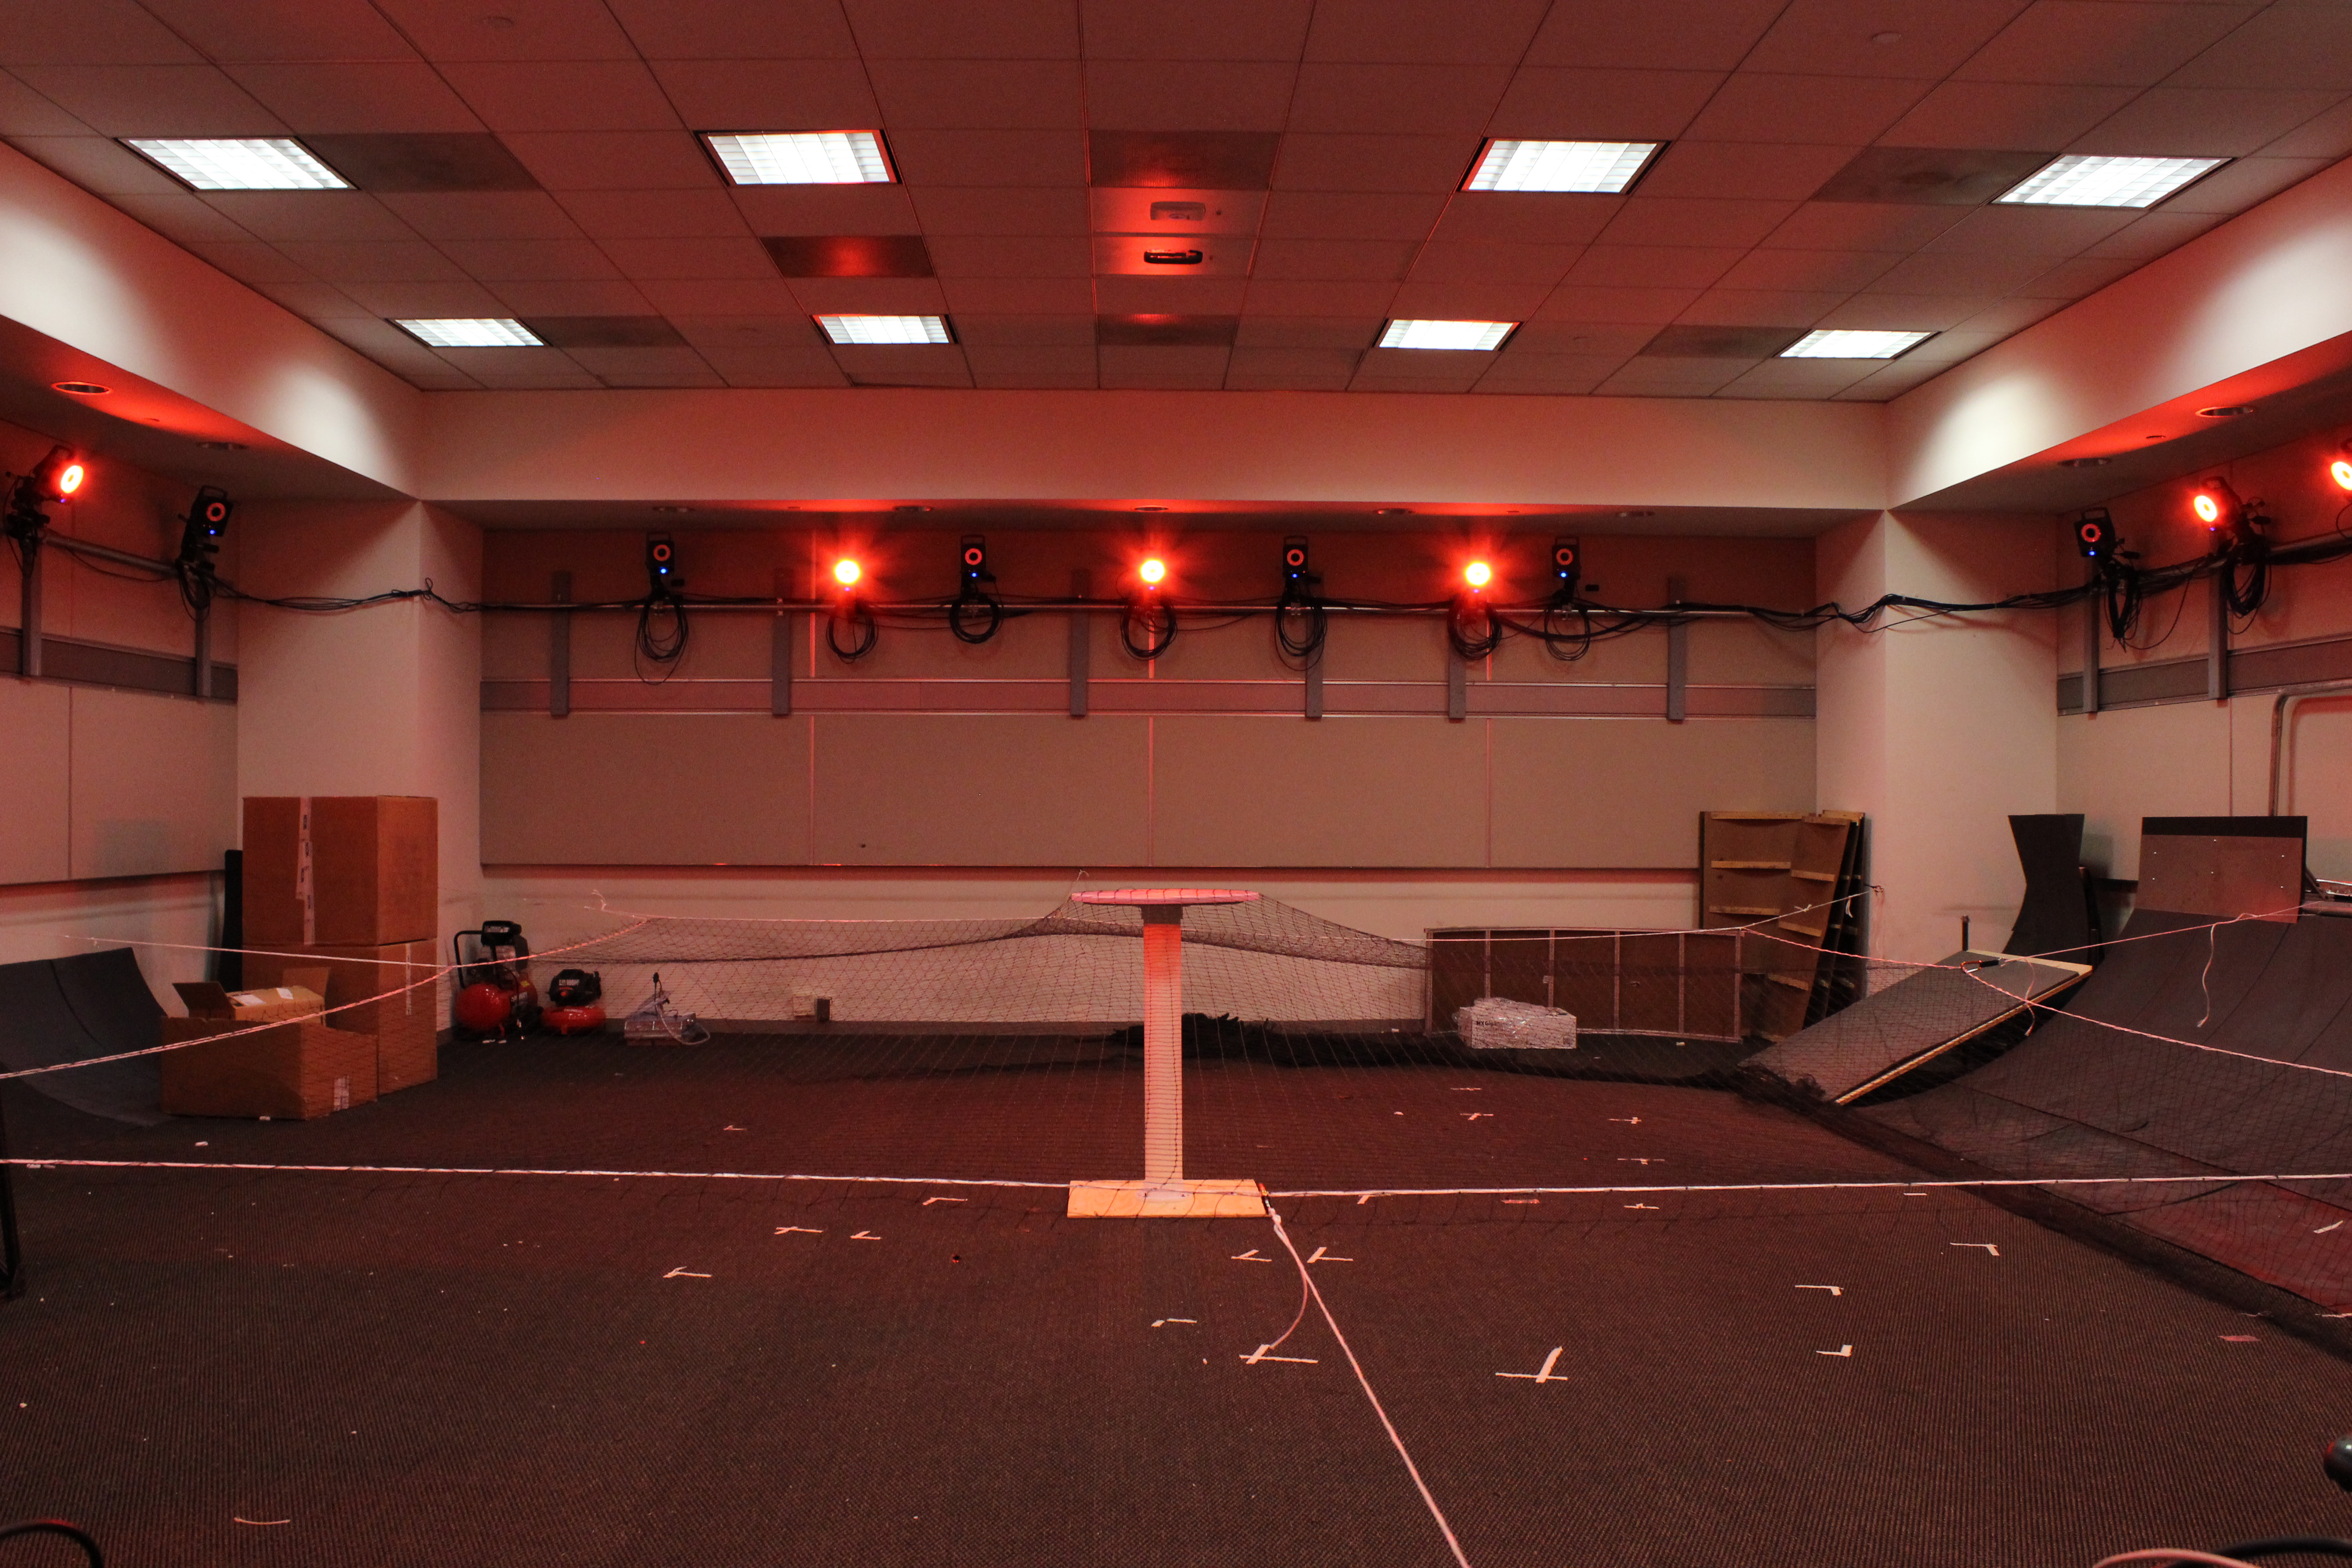
\includegraphics[height=2.5cm]{MoCa}
\vspace*{0.5cm}
}
\end{figure}}
\end{minipage}
}

\end{frame}

\section*{}
\subsection*{Flight Dynamics and Geometric Control}

\begin{frame}
\frametitle{Configuration Space and Dynamics}

\begin{itemize}
\item Local coordinates are completely avoided in the controller design
	\begin{itemize}
	\item Euler angles: any minimal representation of attitude has singularities
	\item Quaternions doublecover $\SO$, yielding an ambiguity
	\end{itemize}
\item Coordinate free approach: configuration space is the special Euclidean group $\SE$ which is the semidirect product of $\Re^3$ and the special orthogonal group ${\SO}=\{R \in{\Re}^{3\times3}\mid R^T R=I,\; \det{R}=1\}$ 
\item Equations of Motion:
\begin{gather*}
\dot x=v,\label{eqn:xdot}\\
m\dot v=mge_3+RF+\Delta_x, \label{eqn:vdot}\\
\dot R=R\hat \Omega,\\
J\dot\Omega + \Omega\times J\Omega =M+\Delta_R\label{eqn:Wdot}
\end{gather*}

\end{itemize}
\end{frame}

\begin{frame}
\frametitle{Geometric Nonlinear Control}

\begin{itemize}
\item Position tracking control is fairly straightforward: linear PID controller applied
\item Attitude control: We define a configuration error function $\Psi:\SO\times\SO\rightarrow\Re$ to yield attitude error function $e_R\in{\Re}^3$ and angular velocity error $e_\Omega\in{\Re}^3$ as follows:
\begin{gather*}
\Psi = \frac{1}{2}{\mathrm{tr}}[G(I-R_d^TR)],\label{eqn:Psi}\\
e_R =\frac{1}{2} (GR_d^TR-R^TR_dG)^\vee,\nonumber
\quad e_\Omega = \Omega - R^T R_d\Omega_d\label{eqn:eW}
\end{gather*}
\item The control force and moment can be derived using these error functions:
\end{itemize}
\begin{gather*}
F = R^T(-k_x e_x-k_v e_v -k_i e_i-mge_3+m\ddot x_d),\label{eqn:F}\\
M = -k_R e_R -k_\Omega e_\Omega -k_I e_I+(R^TR_d\Omega_d)^\wedge J R^T R_d \Omega_d + J R^T R_d\dot\Omega_d\label{eqn:M}
\end{gather*}
\end{frame}

\begin{frame}
\frametitle{Numerical Example}

\only<1>{
\begin{itemize}
\item A desired trajectory where the hexrotor hovers, performs an attitude trajectory where the UAV rotates about is $\vec b_1$ axis, then returns back to its initial attitude and lowers back to its intial position
\item All propeller thrust outputs are within admissible limits:
\begin{figure}
\centerline{
	\subfigure[Position $x, x_d$]{\includegraphics[height=0.25\textwidth]{PositionControl.eps}}
	\hfill
	\subfigure[Attitude $R,R_d$]{\includegraphics[height=0.25\textwidth]{RotationMatrix.eps}}
	\hfill
	\subfigure[Thrust $f,f_{max}$]{\includegraphics[height=0.25\textwidth]{PropellerOutput3by2.eps}}
	}
\end{figure}
\end{itemize}}

\end{frame}



\begin{frame}
\frametitle{Preliminary Experimental Results}

\only<1>{
\begin{itemize}
\item When attached to a swivel stool, the hexrotor is able to follow an attitude trajectory about its yaw axis
\item The geometric PID controller is shown to be robust to disturbances and may handle an impulse
\begin{figure}\setcounter{subfigure}{0}
\centerline{
	\subfigure{\includegraphics[height=0.3\textwidth]{UAV_OnTestStand}}
	\hspace*{0.3cm}
	\subfigure{\includegraphics[height=0.3\textwidth]{Yaw_Test}}
	}
\caption{Hexrotor yaw testing}
\vspace*{-.5cm}
\end{figure}
\item An extended video of yaw testing is available {\bf \href{http://www.youtube.com/watch?v=j0NJP18T1Es&feature=youtu.be}{here}}.
\vspace*{0.5cm}
\end{itemize}
}
\end{frame}

\section*{}
\subsection*{Analysis}

\begin{frame}
\frametitle{Advantages and Disadvantages}

\only<1>{
\begin{itemize}
\item Advantages
\begin{itemize}
\item Free-floating testbed for complex maneuvers
\item Full-actuation to produce a force and moment in any arbitrary direction
\item Large rotational spacecraft maneuver experimentation
\end{itemize}
\item Disadvantages
\begin{itemize}
\item Variable pitch propellers are difficult to control and set
\item Orthogonal propeller plane orientation yields an inefficient design
\item Thrust limitations may prevent hover in some directions:
\end{itemize}
\end{itemize}

\begin{figure}
\centerline{
	\subfigure
		{\includegraphics[width=0.25\columnwidth]{CompletelyAdmissibleRegions}}
	\subfigure
		{\includegraphics[width=0.25\columnwidth]{CompletelyInadmissibleRegions}}
	\subfigure
		{\includegraphics[width=0.25\columnwidth]{PartiallyAdmissibleRegions_connecting}}
	\subfigure
		{\includegraphics[width=0.25\columnwidth]{PartiallyAdmissibleRegions_notconnecting}}
	}
\vspace*{-0.3cm}
\caption{The hexrotor hover may occur when the total thrust (blue cube) is greater than gravity (red sphere) in the body-fixed frame}
\end{figure}
}
\end{frame}

\begin{frame}
\frametitle{Conclusions}

\only<1>{
\begin{itemize}
\item Summary
\begin{itemize}
\item We developed a fully-actuated hexrotor UAV, useful for validating control of spacecraft involving large angle rotational maneuvers
\item We applied a geometric nonlinear controller, capable of performing these maneuvers without linearizing the system dynamics or using local coordinates
\item All mechanical components and communication devices are working properly together
\end{itemize}
\item Future Work
\begin{itemize}
\item Improvements in increasing thrust and reducing mass to maximize the region of admissible hover
\item Development of a hybrid controller to expel the system from dangerous attitude hover regions
\item Spherical joint testing, free floating testing
\end{itemize}
\end{itemize}
}
\end{frame}



%\begin{frame}
%\frametitle{Introduction}
%\begin{itemize}
%    \item Attitude Dynamics of a Rigid Body
%    \begin{itemize}
%    	\item Examples: robotics, flight dynamics, and space systems
%    	\item Attitude: orientation of a body-fixed frame with respect to a reference frame
%		\item Special Orthogonal Group
%        \begin{align*}
%        \SO = \{ R\in\Re^{3\times 3}\,|\, R^TR=I,\quad\mathrm{det}[R]=1\}.
%        \end{align*}
%        \item Compact nonlinear configuration manifold
%        \item Unique dynamic properties that cannot be observed in $\Re^n$
%    \end{itemize}
%\end{itemize}
%
%\only<1->{
%\begin{figure}
%\centerline{
%    \includegraphics[width=2.1cm]{f22.jpg}\hspace*{0.1cm}
%    \includegraphics[width=2.1cm]{sat.jpg}\hspace*{0.1cm}
%    \includegraphics[width=2.1cm]{ast.jpg}\hspace*{0.1cm}
%    \includegraphics[width=2.1cm]{rov.pdf}
%}
%\end{figure}}
%
%\end{frame}
%
%
%\begin{frame}
%\frametitle{Introduction}
%\framesubtitle{Attitude Control Systems: Classification Based on Representation}
%
%\begin{itemize}
%	\item Euler angles
%	\begin{itemize}
%	\item Any minimal representation of attitude has singularities
%	\item Switching between several types to cover $\SO$
%	\item Complex expressions for trigonometric functions
%	\end{itemize}
%\vspace*{0.3cm}\pause
%	\item Quaternions in $\Sph^3=\{q\in\Re^4\,|\, \|q\|=1\}$
%	\begin{itemize}
%	\item No singularities
%	\item Ambiguity: $\Sph^3$ double-covers $\SO$
%	\pause
%	\item Unwinding: a rigid body rotates unnecessarily through a large angle, even if the initial attitude error is small %{\footnotesize [Bhat, Bernstein 00]}
%	\item Sensitive to measurement noise %{\footnotesize [Mayhew et. al. 11]}
%	\pause
%	\item Attitude in $\SO$ should be \emph{carefully} lifted to $\Sph^3$
%	\end{itemize}
%\vspace*{0.3cm}\pause
%	\item Rotation matrices in $\SO$	
%	\begin{itemize}
%	\item No singularity, and no ambiguity
%	\end{itemize}
%\end{itemize}
%
%\end{frame}
%
%
%
%\begin{frame}
%\frametitle{Introduction}
%\framesubtitle{Attitude Control Systems: Classification Based on Stability Properties}
%
%\begin{itemize}
%	\item Topological Obstruction
%	\begin{itemize}
%	\item No \emph{smooth} control system to \emph{globally} asymptotically stabilize a desired attitude
%	\item Region of attraction is homeomorphic to $\Re^n$
%	\end{itemize}
%\vspace*{0.3cm}\pause
%	\item \emph{Almost} Global Asymptotic Stabilization
%	\begin{itemize}
%	\item Smooth control system
%	\item Desired attitude is asymptotically stable
%	\item Region of attraction excludes a zero-measure set
%	\end{itemize}
%\vspace*{0.3cm}\pause
%	\item \emph{Hybrid} Global Asymptotic Stabilization
%	\begin{itemize}
%	\item Hysteresis-based switching control system
%	\item Asymptotic stability from hybrid invariance principle
%	\end{itemize}
%\end{itemize}
%
%\end{frame}
%
%
%
%
%\begin{frame}
%\frametitle{Introduction}
%\framesubtitle{Contributions}
%
%\begin{itemize}
%\item \emph{Exponential} Stability
%	\begin{itemize}
%	\item Prior Work: asymptotic stability
%		\begin{itemize}
%		\item Stabilization: LaSalle's principle
%		\item Tracking: an exogenous system to reformulate it into a hybrid autonomous system
%		\end{itemize} 
%	\item Lyapunov analysis for time-varying systems on $\SO$
%	\end{itemize}
%\vspace*{0.3cm}\pause
%\item Simple Hybrid Control System for \emph{Global} Attractiveness
%	\begin{itemize}
%	\item Prior Work: error function based on stretched rotations, etc
%	\item New intuitive form of attitude error function is introduced for simpler, explicit stability conditions
%	\end{itemize}
%\vspace*{0.3cm}\pause
%\item \emph{Robustness}
%	\begin{itemize}
%	\item Prior Work: integral term is used heuristically without stability analysis
%	\item New integral term is introduced to guarantee stability with fixed disturbances
%	\end{itemize}
%\end{itemize}
%\end{frame}
%
%
%\section*{}
%\subsection*{Problem Formulation}
%
%
%\begin{frame}
%\frametitle{Problem Formulation}
%
%\begin{itemize}
%    \item Attitude Dynamics of a Rigid Body
%    \begin{itemize}
%    \item Equations of motion
%    \begin{gather*}
%J\dot \Omega + \Omega\times J\Omega = u +\Delta,\\
%\dot R = R\hat\Omega = \hat\omega R,\quad (\omega=R\Omega).
%\end{gather*}
%	\item Fixed unknown disturbance: $\Delta\in\Re^3$
%    \end{itemize}
%\vspace*{0.4cm}\pause    
%    \item Attitude Tracking Problem
%    \begin{itemize}
%    \item Desired attitude trajectory: $R_d(t):[t_0,t_f]\rightarrow\SO$
%    \begin{gather*}
%    \dot R_d = R_d \hat\Omega_d = \hat\omega_d R_d,\quad (\omega_d=R_d\Omega_d).
%    \end{gather*}
%    \item Goal: Design control input $u$ such that $(R,\omega)=(R_d,\omega_d)$ is globally exponentially stable
%    \end{itemize}
%\end{itemize}
%\end{frame}
%
%
%\section*{}
%\subsection*{Control Systems Design}
%
%
%\begin{frame}
%\frametitle{Control Systems Design}
%
%\begin{itemize}
%\item Four Types of Attitude Control Systems
%\end{itemize}
%\vspace*{-0.8cm}
%\begin{figure}
%\setlength{\unitlength}{0.1\textwidth}\footnotesize
%\begin{picture}(10,6)(-5.3,-2.8)
%\only<1->{
%%
%\put(-6,0.9){\shortstack[c]{Without\\ disturbance\\ $\Delta=0$}}
%\put(-3.3,2.5){\shortstack[c]{Smooth control}}
%\put(-4.3,0.3){\framebox(4,2)[c]{\shortstack[c]{Smooth Attitude Tracking\\for \textit{Almost Global}\\ \textit{Exponential} Stability}}}}
%%
%\only<2->{
%\put(-0.3,1.3){\vector(1,0){0.8}}
%\put(1.6,2.5){\shortstack[c]{Hybrid control}}
%\put(0.5,0.3){\dashbox{0.08}(4,2)[c]{\shortstack[c]{Hybrid Attitude Tracking\\for \textit{Global}\\ \textit{Exponential} Stability}}}}
%%
%\only<3->{
%\put(-2.3,0.3){\vector(0,-1){0.6}}
%\put(2.5,0.3){\vector(0,-1){0.6}}
%\put(-6,-1.7){\shortstack[c]{With\\ disturbance\\ $\Delta\neq0$}}
%{\linethickness{1.0pt}
%\put(-4.3,-2.3){\framebox(4,2)[c]{\shortstack[c]{Smooth Attitude Tracking\\for \textit{\bf Robust} \textit{Almost Global}\\ \textit{Exponential} Stability}}}}
%{\linethickness{1.0pt}
%\put(0.5,-2.3){\dashbox{0.08}(4,2)[c]{\shortstack[c]{Hybrid Attitude Tracking\\for \textit{{\bf Robust} Global}\\ \textit{Exponential} Stability}}}}}
%\end{picture}
%\end{figure}
%
%\end{frame}
%
%
%\begin{frame}
%\frametitle{Smooth Attitude Tracking}
%
%\begin{itemize}
%\item Attitude Error Function: {\small $\Psi(R,R_d):\SO^2\rightarrow \Re_+$}
%\begin{itemize}
%\item Choose characteristic direction $b_1,b_2\in\Sph^2$ fixed to the body\\
%(ex: direction of an antenna of satellite)
%\item \textit{Current} direction of $b_i$ in the inertial frame: $r_i = R b_i\in\Sph^2$
%\item \textit{Desired} direction of $b_i$ in the inertial frame: $r_{i_d} = R_d b_i\in\Sph^2$
%\item Direction error function: $\Psi_i=\frac{1}{2}\|r_i-r_{i_d}\|^2=1- r_i \cdot r_{i_d}$
%\item Attitude error function:
%\begin{gather*}
%\Psi = k_1 \Psi_1 + k_2 \Psi_2,\quad (k_1\neq k_2).
%\end{gather*}
%\end{itemize}
%\pause\vspace*{0.1cm}
%\item Attitude Error Vector: {\small $e_r(R,R_d):\SO^2\rightarrow \Re^3$}
%	\begin{itemize}
%	\item Derivatives of the error function
%	\begin{align*}
%	\frac{d}{d\epsilon}\bigg|_{\epsilon=0} \Psi(R\exp(\epsilon\hat\eta),R_d) = e_r\cdot \eta.%(R^T r_{i_d}\times b_i)\cdot \eta \equiv e_{r_i}\cdot\eta.
%	\end{align*}
%%	\item Attitude error vector: $e_r = k_1 e_{r_1} + k_2 e_{r_2}$.
%	\end{itemize}
%	\vspace*{0.1cm}
%\pause	
%\item Angular Velocity Error Vector: $e_\Omega=\Omega- R^T\omega_d$.	
%\end{itemize}
%\end{frame}
%
%
%%\begin{frame}
%%\frametitle{Smooth Attitude Tracking}
%%
%%\begin{itemize}
%%\item Angular Velocity Error Vector: $e_\Omega=\Omega- R^T\omega_d$.
%%\end{itemize}
%%
%%\begin{prop}
%%\begin{itemize}\setlength{\itemsep}{0pt}
%%\item[(i)] $\Psi$ is positive definite about $R=R_d$.
%%\item[(ii)] the left-trivialized derivative of $\Psi$ is $\T^*_I \L_R\, (\D_R\Psi(R,R_d))= e_r$.
%%\item[(iii)] $\dot\Psi= e_r\cdot e_\Omega$, $\dot e_r\leq (k_1+k_2)\|e_\Omega\|$.
%%\item[(iv)] there exist $h_1,h_2>0$ such that
%%\begin{align*}
%%h_1\|e_r\|^2 \leq \Psi(R,R_d) \leq h_2 \|e_r\|^2.
%%\end{align*}
%%\end{itemize}
%%\end{prop}
%%\end{frame}
%
%
%\begin{frame}
%\frametitle{Smooth Attitude Tracking}
%
%\begin{itemize}
%\item Smooth Attitude Tracking Control on $\SO$
%
%\begin{prop}\label{prop:AGASSO}
%For $k_1,k_2,k_\omega >0$ with $k_1\neq k_2$ a control input is chosen as
%\begin{align*}
%u & = -e_r -k_\Omega e_\Omega  +(R^T\omega_d)^\wedge JR^T\omega_d
%+ JR^T\dot\omega_d.\label{eqn:uSO}
%\end{align*}
%Then, the following properties hold:
%\begin{enumerate}
%\item There are four equilibrium attitudes, given by $R_d$ and $180^\circ$ rotation of $R_d$ about each of $r_{1_d}$, $r_{2_d}$, and $r_{1_d}\times r_{2_d}$.
%\item The desired attitude is almost globally asymptotically stable and almost semi-globally exponentially stable.
%\item The three undesired equilibria are unstable.
%\end{enumerate}
%\end{prop}
%\end{itemize}
%\end{frame}
%
%
%\begin{frame}
%\frametitle{Numerical Example}
%
%\begin{itemize}
%\item Simulation Parameters
%	\begin{itemize}
%	\item Inertia Matrix: $J=\mathrm{diag}[3,\,2,\,1]\,\mathrm{kgm^2}$.
%	\vspace*{0.3cm}
%	\item Desired Attitude Trajectory
%	\begin{gather*}
%	R_d(t) =\exp(\psi(t)\hat e_3)\exp(\theta(t)\hat e_2)\exp(\phi(t)\hat e_1),\\
%	\phi(t)=\sin 0.5t,\quad \theta(t)=0.1(-1+t),\quad \psi(t)=1-\cos t.
%	\end{gather*}
%	\item Controller Parameters
%	\begin{gather*}
%	k_1=10,\quad k_2=11,\quad k_\Omega=4.42
%	\end{gather*}
%	\end{itemize}
%\end{itemize}
%
%\end{frame}
%
%\begin{frame}
%\frametitle{Numerical Example}
%
%\only<1>{
%\begin{itemize}
%\item Initial Conditions: {\small $R(0)=I$, $\Omega(0)=0_{3\times 1}$ }
%\begin{figure}
%\centerline{
%	\subfigure[Attitude Error $\|R-R_d\|$]{\includegraphics[width=0.47\textwidth]{ACC13_1_neR.pdf}}
%	\hfill
%	\subfigure[Angular Velocity Error $e_\Omega$]{\includegraphics[width=0.47\textwidth]{ACC13_1_eW.pdf}}
%	}
%\end{figure}
%\end{itemize}}
%
%\only<2>{
%\begin{itemize}
%\item Initial Conditions: {\small $R(0) = \exp(0.9999\pi (r_{1_d}\times r_{2_d})^\wedge) R_d(0)$, $\Omega(0)=R(0)^T \omega_d(0)$ (close to one of the undesired equilibria)}
%\begin{figure}\setcounter{subfigure}{0}
%\centerline{
%	\subfigure[Attitude Error $\|R-R_d\|$]{\includegraphics[width=0.47\textwidth]{ACC13_3_neR.pdf}}
%	\hfill
%	\subfigure[Angular Velocity Error $e_\Omega$]{\includegraphics[width=0.47\textwidth]{ACC13_3_eW.pdf}}
%	}
%\end{figure}
%\end{itemize}}
%
%\end{frame}
%
%
%
%\begin{frame}
%\frametitle{Hybrid Attitude Tracking}
%
%\only<1>{
%\begin{itemize}
%\item Smooth Attitude Tracking
%\begin{figure}\setcounter{subfigure}{0}
%\centerline{
%	\subfigure[Error Function $\Psi_i=1-r_i\cdot r_{i_d}$]{\includegraphics[width=0.47\textwidth]{ACC13_H_P0.pdf}}
%	\hfill
%	\subfigure[Error Vector $e_{r_i}$]{\includegraphics[width=0.475\textwidth]{ACC13_H_er0.pdf}}
%	}
%\caption{Direction error function $\Psi_i$ and error vector $e_{r_1}$ as a function of angle between $r_i$ and $r_{i_d}$}
%\end{figure}
%\end{itemize}}
%
%\only<2>{
%\begin{itemize}
%\item Hybrid Attitude Tracking
%\begin{itemize}
%\item Introduce \textbf{\textit{\color{red}{expelling}}} functions: $\Psi_{E_i}=\alpha+\beta r_i\cdot (r_{1_d}\times r_{2_d})$
%\end{itemize}
%\begin{figure}\setcounter{subfigure}{0}
%\centerline{
%	\subfigure[Error Function $\Psi_i,\Psi_{E_i}$]{\includegraphics[width=0.47\textwidth]{ACC13_H_P1.pdf}}
%	\hfill
%	\subfigure[Error Vector $e_{r_i},e_{E_i}$]{\includegraphics[width=0.475\textwidth]{ACC13_H_er1.pdf}}
%	}
%\caption{Direction error function $\Psi_i$ and error vector $e_{r_1}$ as a function of angle between $r_i$ and $r_{i_d}$}
%\end{figure}
%\end{itemize}
%}
%\end{frame}
%
%
%\begin{frame}
%\frametitle{Hybrid Attitude Tracking}
%
%\only<1>{
%\begin{itemize}
%\item Switching Algorithm
%\begin{itemize}
%\item Choose the error function with the minimum value
%\item Sensitive to noise, chattering
%\end{itemize}
%\begin{figure}\setcounter{subfigure}{0}
%\centerline{
%	\subfigure[Error Function $\Psi_i,\Psi_{E_i}$]{\includegraphics[width=0.47\textwidth]{ACC13_H_P2.pdf}}
%	\hfill
%	\subfigure[Error Vector $e_{r_i},e_{E_i}$]{\includegraphics[width=0.475\textwidth]{ACC13_H_er2.pdf}}
%	}
%\caption{Direction error function $\Psi_i$ and error vector $e_{r_1}$ as a function of angle between $r_i$ and $r_{i_d}$}
%\end{figure}
%\end{itemize}}
%
%
%\only<2>{
%\begin{itemize}
%\item Hysteresis-Based Switching Algorithm
%\begin{itemize}
%\item Switch if the difference to the min. value is greater than $\delta$
%\item Robust to noise, eliminate chattering
%\end{itemize}
%\begin{figure}\setcounter{subfigure}{0}
%\centerline{
%	\subfigure[Error Function $\Psi_i,\Psi_{E_i}$]{\includegraphics[width=0.47\textwidth]{ACC13_H_P3.pdf}}
%	\hfill
%	\subfigure[Error Vector $e_{r_i},e_{E_i}$]{\includegraphics[width=0.475\textwidth]{ACC13_H_er3.pdf}}
%	}
%\caption{Direction error function $\Psi_i$ and error vector $e_{r_1}$ as a function of angle between $r_i$ and $r_{i_d}$}
%\end{figure}
%\end{itemize}}
%
%
%\end{frame}
%
%\begin{frame}
%\frametitle{Hybrid Attitude Tracking}
%
%\begin{itemize}
%\item Global Exponential Attitude Tracking on $\SO$
%
%\begin{prop}\label{prop:GES}
%Consider the hybrid control system described above. For given constants $k_1,k_2,\alpha,\beta$ satisfying $k_1,k_2>0$, $k_1\neq k_2$, $1<\alpha<2$ and $|\beta|< \alpha-1$, choose the hysteresis gap $\delta$ such that
%\begin{align}
%0<\delta < \min\{k_1,k_2\}\min\{2-\alpha, \alpha-|\beta|-1\}.\label{eqn:deltaSO}
%\end{align}
%Then, the desired equilibrium $(R_d,\omega_d)$ is globally exponentially stable.
%\end{prop} 
%
%\begin{itemize}
%\item Sufficient condition for stability is \emph{explicitly} given by (1)
%\item Stronger global \emph{exponential} stability is guaranteed
%\end{itemize}
%\end{itemize}
%\end{frame}
%
%
%
%\begin{frame}
%\frametitle{Numerical Example}
%
%\only<1>{
%\begin{itemize}
%\item Smooth Attitude Control
%\begin{itemize}
%\item Initial Conditions: {\small $R(0) = \exp(0.9999\pi (r_{1_d}\times r_{2_d})^\wedge) R_d(0)$, $\Omega(0)=R(0)^T \omega_d(0)$ (close to one of the undesired equilibria)}
%\end{itemize}
%\begin{figure}\setcounter{subfigure}{0}
%\centerline{
%	\subfigure[Attitude Error $\|R-R_d\|$]{\includegraphics[width=0.47\textwidth]{ACC13_3_neR.pdf}}
%	\hfill
%	\subfigure[Angular Velocity Error $e_\Omega$]{\includegraphics[width=0.47\textwidth]{ACC13_3_eW.pdf}}
%	}
%\end{figure}
%\end{itemize}}
%
%
%\only<2>{
%\begin{itemize}
%\item Hybrid Attitude Control
%\begin{itemize}
%\item Initial Conditions: {\small $R(0) = \exp(0.9999\pi (r_{1_d}\times r_{2_d})^\wedge) R_d(0)$, $\Omega(0)=R(0)^T \omega_d(0)$ (close to one of the undesired equilibria)}
%\end{itemize}
%\begin{figure}\setcounter{subfigure}{0}
%\centerline{
%	\subfigure[Attitude Error $\|R-R_d\|$]{\includegraphics[width=0.47\textwidth]{ACC13_4_neR.pdf}}
%	\hfill
%	\subfigure[Angular Velocity Error $e_\Omega$]{\includegraphics[width=0.47\textwidth]{ACC13_4_eW.pdf}}
%	}
%\end{figure}
%\end{itemize}}
%
%
%\end{frame}
%
%
%
%\begin{frame}
%\frametitle{Control Systems Design}
%
%\begin{itemize}
%\item Four Types of Attitude Control Systems
%\end{itemize}
%\vspace*{-0.8cm}
%\begin{figure}
%\setlength{\unitlength}{0.1\textwidth}\footnotesize
%\begin{picture}(10,6)(-5.3,-2.8)
%\only<1->{
%%
%\put(-6,0.9){\shortstack[c]{Without\\ disturbance\\ $\Delta=0$}}
%\put(-3.3,2.5){\shortstack[c]{Smooth control}}
%\put(-4.3,0.3){\framebox(4,2)[c]{\shortstack[c]{Smooth Attitude Tracking\\for \textit{Almost Global}\\ \textit{Exponential} Stability}}}}
%%
%\only<1->{
%\put(-0.3,1.3){\vector(1,0){0.8}}
%\put(1.6,2.5){\shortstack[c]{Hybrid control}}
%\put(0.5,0.3){\dashbox{0.08}(4,2)[c]{\shortstack[c]{Hybrid Attitude Tracking\\for \textit{Global}\\ \textit{Exponential} Stability}}}}
%%
%\only<2->{
%\put(-2.3,0.3){\vector(0,-1){0.6}}
%\put(2.5,0.3){\vector(0,-1){0.6}}
%\put(-6,-1.7){\shortstack[c]{With\\ disturbance\\ $\Delta\neq0$}}
%{\linethickness{1.0pt}
%\put(-4.3,-2.3){\framebox(4,2)[c]{\shortstack[c]{Smooth Attitude Tracking\\for \textit{\bf Robust} \textit{Almost Global}\\ \textit{Exponential} Stability}}}}
%{\linethickness{1.0pt}
%\put(0.5,-2.3){\dashbox{0.08}(4,2)[c]{\shortstack[c]{Hybrid Attitude Tracking\\for \textit{{\bf Robust} Global}\\ \textit{Exponential} Stability}}}}}
%\end{picture}
%\end{figure}
%
%\end{frame}
%
%
%\begin{frame}
%\frametitle{Robust Attitude Tracking}
%
%\begin{itemize}
%\item Generalized Integral Term
%\begin{itemize}
%\item Definition
%
%\begin{center}\hspace*{0.01cm}
%\begin{beamercolorbox}[wd=8cm,dp=0.15cm,ht=1.1cm,sep=0.05cm,center,shade=on]{numerical}
%$e_I(t) = \displaystyle\int_{0}^t ce_r(\tau)+e_\Omega(\tau) \,d\tau.$
%\end{beamercolorbox}
%\end{center}
%
%%
%%
%%\begin{align}
%%e_I(t) = \int_{0}^t ce_r(\tau)+e_\Omega(\tau) \,d\tau,\label{eqn:eI}
%%\end{align}
%%for some positive constant $c$.
%\item The first part is equivalent to the \textit{classical} integral term
%\item The second term increases the proportional term effectively\\
%(Note: $\dot e_r \neq e_\Omega$) 
%\pause\vspace*{0.3cm}
%\item Control inputs are augmented with the proposed, generalized integral term
%\item Stabilities are guaranteed by rigorous Lyapunov analysis for time-varying systems
%\end{itemize}
%\end{itemize}
%\end{frame}
%
%
%\begin{frame}
%\frametitle{Robust Attitude Tracking}
%
%\begin{itemize}
%\item Smooth Attitude Tracking
%\begin{prop}\label{prop:RAGAS}
%Control input is chosen as
%{\small
%\begin{align*}
%u & = -e_r -k_\Omega e_\Omega -k_I e_I+(R^T\omega_d)^\wedge JR^T\omega_d
%+ JR^T\dot\omega_d.\label{eqn:uI}
%\end{align*}}
%Then, the desired equilibrium is almost globally asymptotically stable, and locally exponentially stable with respect to $e_r,e_\Omega$. The integral term $e_I$ is globally uniformly bounded.
%\end{prop}
%\pause\vspace*{0.1cm}
%\item Hybrid Attitude Tracking
%\begin{prop}
%The desired equilibrium $(R_d,\omega_d)$ is globally exponentially stable with respect to $e_r$ and $e_\Omega$, and the integral term $e_{I}$ is globally uniformly bounded.
%\end{prop}
%\end{itemize}
%
%\end{frame}
%
%
%\begin{frame}
%\frametitle{Numerical Example}
%
%\only<1>{
%\begin{itemize}
%\item Hybrid Attitude Control
%\begin{itemize}
%\item Initial Conditions: {\small $R(0) = \exp(0.9999\pi (r_{1_d}\times r_{2_d})^\wedge) R_d(0)$, $\Omega(0)=R(0)^T \omega_d(0)$ (close to one of the undesired equilibria)}
%\item Fixed Disturbance: $\Delta=[-1,2,1]^T$.
%\end{itemize}
%\begin{figure}\setcounter{subfigure}{0}
%\centerline{
%	\subfigure[Attitude Error $\|R-R_d\|$]{\includegraphics[width=0.47\textwidth]{ACC13_7_neR.pdf}}
%	\hfill
%	\subfigure[Angular Velocity Error $e_\Omega$]{\includegraphics[width=0.47\textwidth]{ACC13_7_eW.pdf}}
%	}
%\end{figure}
%\end{itemize}}
%
%
%\only<2>{
%\begin{itemize}
%\item Robust Hybrid Attitude Control
%\begin{itemize}
%\item Initial Conditions: {\small $R(0) = \exp(0.9999\pi (r_{1_d}\times r_{2_d})^\wedge) R_d(0)$, $\Omega(0)=R(0)^T \omega_d(0)$ (close to one of the undesired equilibria)}
%\item Fixed Disturbance: $\Delta=[-1,2,1]^T$.
%\end{itemize}
%\begin{figure}\setcounter{subfigure}{0}
%\centerline{
%	\subfigure[Attitude Error $\|R-R_d\|$]{\includegraphics[width=0.47\textwidth]{ACC13_8_neR.pdf}}
%	\hfill
%	\subfigure[Angular Velocity Error $e_\Omega$]{\includegraphics[width=0.47\textwidth]{ACC13_8_eW.pdf}}
%	}
%\end{figure}
%\end{itemize}}
%\end{frame}
%
%
%\section*{}
%\subsection*{Conclusions}
%
%\begin{frame}
%\frametitle{Conclusions}
%\begin{itemize}
%    \item Robust Global Exponential Attitude Tracking
%    \begin{itemize}
%        \item Lyapunov stability analysis for time-varying systems
%        \item Hybrid attitude control with simpler controller design
%        \item Robust control with new generalized integral control term
%    \end{itemize}
%\vspace*{0.4cm}\pause
%    \item Geometric Controls on $\SO$
%    \begin{itemize}
%        \item \textit{Coordinate-free} nonlinear controls on a nonlinear manifold.
%        \item Completely avoid \textit{singularities, ambiguities, and complexities}
%        \item No need to introduce exogenous system to lift $\SO$ to $\Sph^3$
%    \end{itemize}
%\end{itemize}
%\end{frame}



\end{document}

